%This is a \LaTeX\  template created following the Project Report Guidelines of the Examination Office at the International University of Applied Sciences. Please review carefully if all the details in this template are the same as those stated in the official guidelines. Always follow the official guidelines first rather than this template. If you find inconsistencies between the official guideline and this template, please report them to gissel.velarde@iu.org.
%Author: Gissel Velarde

\documentclass[11pt,a4paper]{article}

%\usepackage[margin=2cm]{geometry} % full-width
\usepackage[left=2cm,right=2cm,top=2cm,bottom=2cm]{geometry}
\usepackage[utf8]{inputenc}

\usepackage{setspace}
\onehalfspacing % Set line spacing to 1.5

\usepackage{helvet} %arial font
\renewcommand{\familydefault}{\sfdefault}

\usepackage{sectsty}
\usepackage{graphicx}

\usepackage[hidelinks]{hyperref} 
\usepackage{apacite} %APA style citation, make sure it comes after hyperref!

\usepackage{amsmath, amssymb, latexsym}

%packages for drawings
\usepackage{tikz}
\usetikzlibrary{decorations.pathreplacing}
\usetikzlibrary{fadings}

%\usepackage[style=apa, backend=biber]{biblatex}
%\addbibresource{references.bib}

\setlength\parindent{0pt} %https://tex.stackexchange.com/questions/27802/set-noindent-for-entire-file

%\usepackage{ragged2e} %justified
%\justifying


\title{PROJECT REPORT LATEX TEMPLATE}
\author{ Gissel Velarde }
%\date{\today}

\begin{document}

\maketitle	

% TOC
 \tableofcontents
 \pagebreak

%--Paper--
\section{INTRODUCTION}
This is a \LaTeX\  template created following the Project Report Guidelines of the Examination Office at the International University of Applied Sciences. Please review carefully if all the details in this template are the same as those in the official guidelines. 

\subsection{Content}
In general, reports:

\begin{itemize}
\item introduce a topic, explaining the motivation and goals of the work, 
\item describe the method, 
\item  present the results, and
\item conclude discussing the implications of the work.
\end{itemize}

\section{EXAMPLES}
The captions of tables and figures should clearly explain the presented content, see for example Table \ref{table:1} and Figure \ref{fig:1}. Next, an example of a mathematical expression, where $x$ is the input to a Rectified Linear Unit (ReLU) activation function \shortcite{goodfellow2016deep}:

\begin{equation} \label{e:1}
f(x)=max(0,x). 
\end{equation}

Finally, this is how you cite a book \cite{velarde2023artificial}, an article \cite{lecun1989handwritten}, and online material \cite{Stutz2022}.\footnote{Please avoid using footnotes.} 

\begin{table}[h!]
\centering
\begin{tabular}{|c c|} 
 \hline
Study program &  Report length \\  \hline
BACHELOR &  7 -- 10  pages of text  \\ 
MASTER  & 12 -- 15 pages of text\\

 \hline
\end{tabular}
\caption{Length of reports in number of pages according to the study program.}
\label{table:1}
\end{table}

\begin{figure}[h]
	\centering
	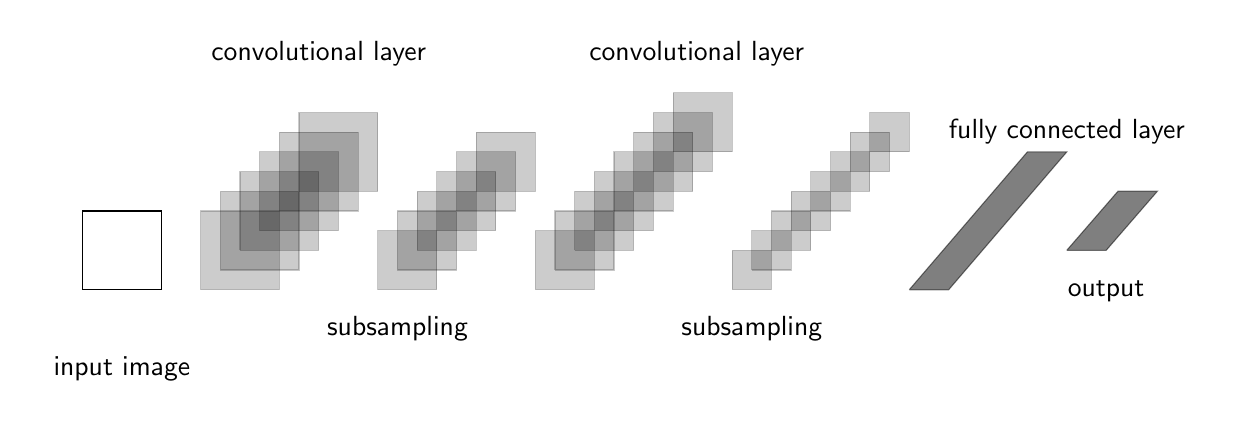
\begin{tikzpicture}
		\node at (0.5,-1){\begin{tabular}{c}input image\end{tabular}};
		
		\draw (0,0) -- (1,0) -- (1,1) -- (0,1) -- (0,0);
		
		\node at (3,3){\begin{tabular}{c}convolutional layer\end{tabular}};
		
		\draw[fill=black,opacity=0.2,draw=black] (2.75,1.25) -- (3.75,1.25) -- (3.75,2.25) -- (2.75,2.25) -- (2.75,1.25);
		\draw[fill=black,opacity=0.2,draw=black] (2.5,1) -- (3.5,1) -- (3.5,2) -- (2.5,2) -- (2.5,1);
		\draw[fill=black,opacity=0.2,draw=black] (2.25,0.75) -- (3.25,0.75) -- (3.25,1.75) -- (2.25,1.75) -- (2.25,0.75);
		\draw[fill=black,opacity=0.2,draw=black] (2,0.5) -- (3,0.5) -- (3,1.5) -- (2,1.5) -- (2,0.5);
		\draw[fill=black,opacity=0.2,draw=black] (1.75,0.25) -- (2.75,0.25) -- (2.75,1.25) -- (1.75,1.25) -- (1.75,0.25);
		\draw[fill=black,opacity=0.2,draw=black] (1.5,0) -- (2.5,0) -- (2.5,1) -- (1.5,1) -- (1.5,0);
		
		\node at (4,-0.5){\begin{tabular}{c}subsampling\end{tabular}};
		
		\draw[fill=black,opacity=0.2,draw=black] (5,1.25) -- (5.75,1.25) -- (5.75,2) -- (5,2) -- (5,1.25);
		\draw[fill=black,opacity=0.2,draw=black] (4.75,1) -- (5.5,1) -- (5.5,1.75) -- (4.75,1.75) -- (4.75,1);
		\draw[fill=black,opacity=0.2,draw=black] (4.5,0.75) -- (5.25,0.75) -- (5.25,1.5) -- (4.5,1.5) -- (4.5,0.75);
		\draw[fill=black,opacity=0.2,draw=black] (4.25,0.5) -- (5,0.5) -- (5,1.25) -- (4.25,1.25) -- (4.25,0.5);
		\draw[fill=black,opacity=0.2,draw=black] (4,0.25) -- (4.75,0.25) -- (4.75,1) -- (4,1) -- (4,0.25);
		\draw[fill=black,opacity=0.2,draw=black] (3.75,0) -- (4.5,0) -- (4.5,0.75) -- (3.75,0.75) -- (3.75,0);
		
		\node at (7.8,3){\begin{tabular}{c}convolutional layer\end{tabular}};
		
		\draw[fill=black,opacity=0.2,draw=black] (7.5,1.75) -- (8.25,1.75) -- (8.25,2.5) -- (7.5,2.5) -- (7.5,1.75);
		\draw[fill=black,opacity=0.2,draw=black] (7.25,1.5) -- (8,1.5) -- (8,2.25) -- (7.25,2.25) -- (7.25,1.5);
		\draw[fill=black,opacity=0.2,draw=black] (7,1.25) -- (7.75,1.25) -- (7.75,2) -- (7,2) -- (7,1.25);
		\draw[fill=black,opacity=0.2,draw=black] (6.75,1) -- (7.5,1) -- (7.5,1.75) -- (6.75,1.75) -- (6.75,1);
		\draw[fill=black,opacity=0.2,draw=black] (6.5,0.75) -- (7.25,0.75) -- (7.25,1.5) -- (6.5,1.5) -- (6.5,0.75);
		\draw[fill=black,opacity=0.2,draw=black] (6.25,0.5) -- (7,0.5) -- (7,1.25) -- (6.25,1.25) -- (6.25,0.5);
		\draw[fill=black,opacity=0.2,draw=black] (6,0.25) -- (6.75,0.25) -- (6.75,1) -- (6,1) -- (6,0.25);
		\draw[fill=black,opacity=0.2,draw=black] (5.75,0) -- (6.5,0) -- (6.5,0.75) -- (5.75,0.75) -- (5.75,0);
		
		\node at (8.5,-0.5){\begin{tabular}{c}subsampling\end{tabular}};
		
		\draw[fill=black,opacity=0.2,draw=black] (10,1.75) -- (10.5,1.75) -- (10.5,2.25) -- (10,2.25) -- (10,1.75);
		\draw[fill=black,opacity=0.2,draw=black] (9.75,1.5) -- (10.25,1.5) -- (10.25,2) -- (9.75,2) -- (9.75,1.5);
		\draw[fill=black,opacity=0.2,draw=black] (9.5,1.25) -- (10,1.25) -- (10,1.75) -- (9.5,1.75) -- (9.5,1.25);
		\draw[fill=black,opacity=0.2,draw=black] (9.25,1) -- (9.75,1) -- (9.75,1.5) -- (9.25,1.5) -- (9.25,1);
		\draw[fill=black,opacity=0.2,draw=black] (9,0.75) -- (9.5,0.75) -- (9.5,1.25) -- (9,1.25) -- (9,0.75);
		\draw[fill=black,opacity=0.2,draw=black] (8.75,0.5) -- (9.25,0.5) -- (9.25,1) -- (8.75,1) -- (8.75,0.5);
		\draw[fill=black,opacity=0.2,draw=black] (8.5,0.25) -- (9,0.25) -- (9,0.75) -- (8.5,0.75) -- (8.5,0.25);
		\draw[fill=black,opacity=0.2,draw=black] (8.25,0) -- (8.75,0) -- (8.75,0.5) -- (8.25,0.5) -- (8.25,0);
		
		\node at (12.5,2){\begin{tabular}{c}fully connected layer\end{tabular}};
		
		\draw[fill=black,draw=black,opacity=0.5] (10.5,0) -- (11,0) -- (12.5,1.75) -- (12,1.75) -- (10.5,0);
		
		\node at (13,0){\begin{tabular}{c}output \end{tabular}};
		
		\draw[fill=black,draw=black,opacity=0.5] (12.5,0.5) -- (13,0.5) -- (13.65,1.25) -- (13.15,1.25) -- (12.5,0.5);
	\end{tikzpicture}
	\caption[Architecture of a two-layered convolutional neural network.]{Architecture of a convolutional neural network by \citeA{lecun1989handwritten}. This network has two convolutional layers, each followed by a subsampling layer. A fully connected layer precedes the output layer.  The latex code for this image was adapted from \cite{Stutz2022}.}
	\label{fig:1}
\end{figure}

\section{CONCLUSION}
This template should help you get started with your report. Remember to double-check with the format of the official guidelines.

%the bibliography
\bibliographystyle{apacite}
\bibliography{references.bib}

%--/Paper--

\end{document}